\documentclass[11pt]{report}
\usepackage{graphicx}
%\usepackage{mathptmx}
\topmargin -1.5cm
\oddsidemargin -0.04cm
\evensidemargin -0.04cm
\textwidth 16.59cm
\textheight 21.94cm
\parskip 7.2pt

\begin{document}
%%%%%%%%%%%%%
%
%	TOP MATTER
%
%%%%%%%%%%%%%

\begin{titlepage}
\begin{center}

\textsc{\LARGE Delft University of Technology}\\[1.5cm]

\textsc{\Huge Laser Swarm}\\[0.5cm]
\textsc{\small Project Plan}\\[1.5cm]
\textsc{\large Design Synthesis Exercise}\\[2.5cm]

\begin{minipage}{0.4\textwidth}
\begin{flushleft} \large
\emph{Authors:}\\
\textsc{S. Billemont\\
L.S. Boersma\\
B. Buyens\\
S.R. Finck\\
J.P. Florijn\\
T.C. Goossens\\
N.S. Oborin\\
A.J. Vorobiev\\
G.J. van der Wel\\
Z. Zhou\\}
\end{flushleft}
\end{minipage}
\begin{minipage}{0.4\textwidth}
\begin{flushright}
\emph{Tutor:}\\
\textsc{Ben Gorte}\\[1cm]
\emph{Coaches:}\\
\textsc{Prem Sundaramoorthy\\
Mathieu Willaert}
\end{flushright}
\end{minipage}
\vfill

\today
\end{center}
\end{titlepage}

%%%%%%%%%%%%%
%
%	ABSTRACT
%
%%%%%%%%%%%%%

\begin{abstract}
Abstract text goes here
\end{abstract}

%%%%%%%%%%%%%
%
%	TOC
%
%%%%%%%%%%%%%

\tableofcontents

%%%%%%%%%%%%%
%
%	GENERAL SUMMARY
%
%%%%%%%%%%%%%

\chapter{General Summary}
\label{dseSummary}
%Intro
\section{Introduction}
\label{dsePPIntro}
Introduction to dse project plan
%MNS
\section{Mission Need Statement}
\label{dsePPMNS}
Demonstrate that a satellite constellation, consisting of a single emitter and several receivers, will perform better (in terms of cost, lifetime and results) than existing systems.
%POS
\section{Project Objective Statement}
\label{dsePPPOS}
To design a satellite constellation of a single LiDAR emitter and a swarm of receivers, with a team of 10 people. Verify the results using an advanced simulation.
%Requirements
\section{Requirements}
\label{dsePPRequirements}
The requirements go here
%System Description
\section{System Description}
\label{dsePPSystemDescription}
The system under consideration for this project consists of a single LiDAR emitter satellite surrounded by a swarm of receivers. This system may replace the current system of bulky high energy lasers with large receiver telescopes. Contrary to the current system the swarm uses a high frequency, low energy laser combined with a lot of small, very sensitive, receivers in an orbit near the emitter. The receivers have to be able to distinguish single photons that reflect back from the Earth surface. This data is then used to reconstruct the topology of the scanned area.

%%%%%%%%%%%%%
%
%	DSE PROJECT PLAN
%
%%%%%%%%%%%%%

\chapter{Technical Design Development}
\label{dse}
% DSE WFD
\section{Work Flow Diagram}
\label{dsePPWFD}
The work flow diagrams
% DSE WBS
\section{Work Breakdown Structure}
\label{dsePPWBS}
The work breakdown
% DSE Project Approach Description
\section{Project Approach Description}
\label{dseProjectApproachDescription}
The DSE project is approached by first establishing specific roles for the group members, here every group member is assigned a clearly defined management and technical function. After this the group operational procedures are defined. They are as follows:

\begin{enumerate}
	\item The Chairman will lead a scrum meeting every morning upon arrival of all members to establish what everyone has done the day before and what they will be doing the day of the meeting. This is done in order to keep all members up-to-date with all aspects of the project. The meeting concludes with updates on any external communications (with organizations and teaching staff) as well as any other points relevant at that time.
	\item Whenever relevant, groups responsible for certain design tasks should present their results to the rest of the group.
	\item A meeting with the tutor and coaches is held every week and before important deliverables.
	\item Upon completion of a deliverable, a meeting is booked to establish a plan for the next deliverable.  
\end{enumerate}

The official start of the DSE project is marked with the establishment of the Mission Need Statement. At this point all members should be aware of what the main goal of the assignment is.

The design process is started by defining the tasks in the project plan, then finding the requirements and functions. From the requirements, a set of design options will be created before the Mid Term Review (MTR) and based on an extensive functional and risk assessment a trade-off will be made. After the MTR, work on the detailed design can begin. At this stage all subsystems will be given a careful consideration in terms of budgets. Final decisions on detailed parameters and variables will be made. Leading up to the Final Review (FR), the feasibility study can be concluded based on earlier decisions.

Parallel to the design phase, the simulator software will be developed by a team of 3 to 4 people (depending on the time available). This software should be able to perform accurate enough calculations to aid the trade-off scheduled before the MTR.
% DSE OBS
\section{Organizational Breakdown Structure}
\label{dsePPOBS}
The org breakdown

\newpage
\begin{center}
\begin{figure}[H]
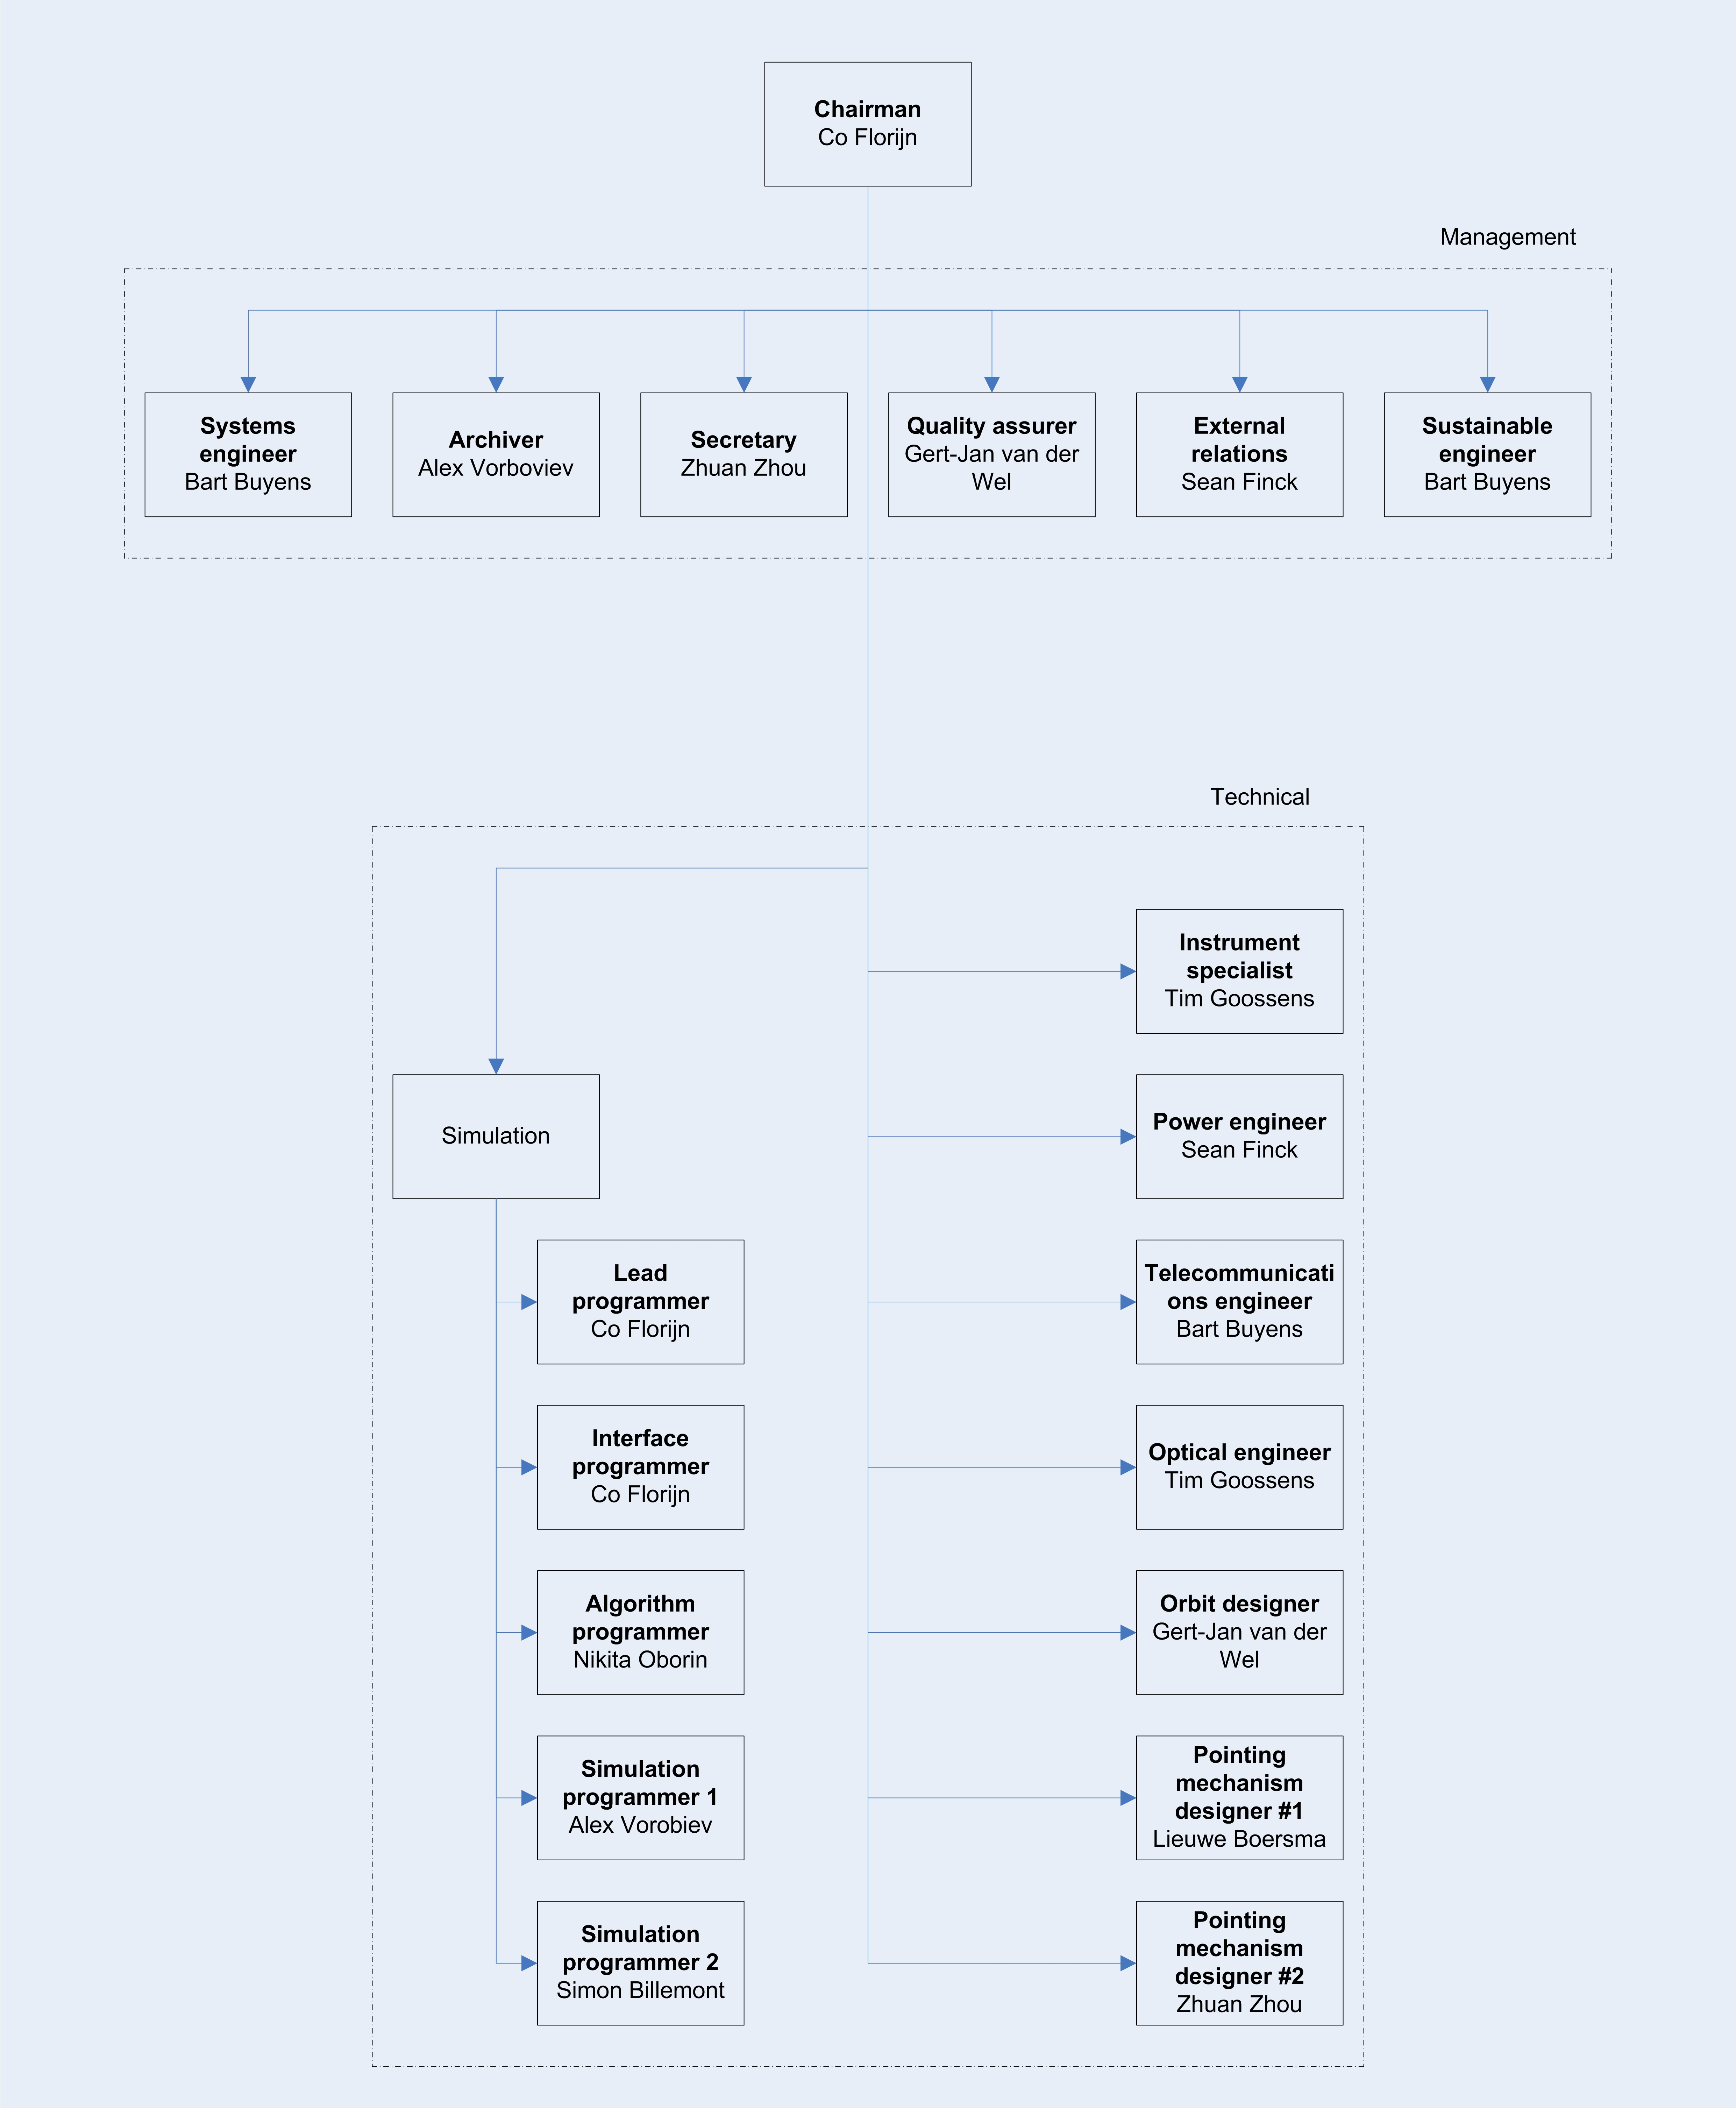
\includegraphics[width=1.2\textwidth]{chapters/img/Organogram.jpg}
\caption{Organogram}
\end{figure}
\end{center}
% DSE Timeline
\section{Timeline}
\label{dsePPTimeline}
The Gantt chart that can be seen in Appendix \ref{ganttchart}
shows the time line of the DSE project.
As can be seen there are four phases. 

The first phase is the start-up of the project. Time is taken here to get to know the project and to
determine the tasks to be done. A team organization is also created and a timeline is made.
The second phase contains the start of the design of the system. The different subsystems are looked 
at individually to better fulfill the requirements. Different design options will be considered.
At the same time the risk assessment, Reliability Availability Maintainability and Safety (RAMS) characteristics and return on investment will be investigated.

During the third phase, three concrete design options will be chosen. Their designs will be elaborated on further.

At the end, a trade-off will be performed according to certain trade-off criteria.
The chosen design will be worked out completely in the last phase. Each subsystem will be completely designed
and integrated into the full system. Lastly the feasibility of the system will be evaluated.
% DSE Risk Management Plan
\section{Risk management plan}
\label{dsePPRiskMP}
This chapter contains the risk management plan. First the possible risks are identified and in the next section they are prioritized. The final section demonstrates some ways to reduce the probability of the highest priority risks. This last section will also show contingency plans in case things do go wrong.
\subsection{Risk identification}
This section contains a list of possible management risks.
\begin{enumerate}
	\item Failure to make the deadline for the project plan.
	\item Failure to make the deadline for the baseline report.
	\item Failure to make the deadline for the mid-term report.
	\item Failure to make the deadline for the final report.
	\item Failure to make the deadline for the symposium.
	\item Simulation is delayed.
	\item Several tasks are not completed on time.
	\item Team member is late.
	\item Absence of a team member.
	\item Unscheduled absence of the tutor or coaches.
	\item External emergency, e.g. fire/power outage.
	\item Someone is unable to properly perform his designated management function.
\end{enumerate}
\subsection{Risk prioritisation}
The risks will be assigned a probability and impact to determine the highest risk event. The numbers in the following list correspond to the numbers in the previous section.
\begin{enumerate}
	\item The impact is severe, because the deadlines are set by the DSE organization. The probability of occurrence is medium because of the time limit.
	\item The impact and probability of this point is the same as for the first.
	\item The impact and probability of this point is the same as for the first.
	\item The impact and probability of this point is the same as for the first.
	\item The impact of not making this deadline is severe because a lot of people will be disappointed. The probability of occurrence is negligible, as six days are available to make the presentation.
	\item The impact of this event is high, as the simulation is required on several occasions like the trade-off and the final report. The probability of occurrence is low as three people are working on it the whole time.
	\item The impact is severe because people will have to be pulled from their own tasks for an extended period of time. The probability of occurrence is low. If one task is delayed it is possible others are as well.
	\item The impact is low as it may be possible for the team member to catch up on the same day. The probability of occurrence is medium because it is possible for someone to, for example, miss his train.
	\item The impact is high because that means someone else will have to do the work of the absent team member. The probability of occurrence is negligible, it is unlikely a member falls ill. Other reasons should not play a role, as defined by the regulations for the DSE.
	\item The impact is low as other people can be asked instead. The probability of occurrence is negligible, absence will be announced ahead of time whenever possible. It is just as unlikely for a coach or tutor to fall ill as for a group member, so this probability is negligible as well.
	\item The impact is severe as it will most likely mean at least a day will be lost, in the worst case all our possessions or work are lost. The probability of occurrence is extremely negligible.
	\item The impact is high as it can seriously degrade the report. The probability of occurrence is low, as the assigned tasks are to be taken seriously.
\end{enumerate}

\begin{table}
	\centering
		\begin{tabular}{c|c||c|c|c|c|}
		\multicolumn{2}{c||}{} & \multicolumn{4}{|c|}{probability of occurrence} \\ \cline{3-6}
		\multicolumn{2}{c||}{} & negligible & low & medium & high \\ \hline \hline
		\multirow{5}{*}{consequences} & severe & 5,11 & 7 & 1,2,3,4 &  \\ \cline{2-6}
		 & high & 9 & 6,12 &  &  \\ \cline{2-6}
		 & medium & & & & \\ \cline{2-6}
		 & low & 10 & & 8 & \\ \cline{2-6}
		 & negligible & & & & \\
		\hline
	\end{tabular}
	\caption{Risk management matrix}
	\label{tab:Riskmanagementmatrix}
\end{table}

As can be seen in Table-\ref{tab:Riskmanagementmatrix} cases 1,2,3,4 are the highest risk cases followed closely by cases 7,6 and 12. Several ways to reduce the risks are defined in the next section.

\subsection{Risk reduction and contingency plans}
The risks for cases 1 to 4 can be reduced by strictly enforcing a project plan that is set up during both the first week of the project and at the beginning of the period where the mid-term report has to be made. The project plan is also of great benefit to sections 6 and 7. For 12 the only thing that can be done to reduce the probability is to check whether the functions are performed properly at regular intervals during the exercise.

In case things do go wrong on points 6 and 7 the most obvious thing to do is to continue working into the evening to finish the job. It may also be possible to reassign people to another tasks. Cases 1 to 4 are fixed deadlines, if they are not made then a penalty will be placed on the report. The only solution possible is to finish the report as soon as possible so there is as little delay as possible for the next deliverable. If a case 12 is detected the person has to be made aware of his error (or errors), and if that does not work a replacement has to be found.

%%%%%%%%%%%%%
%
%	SUSTAINABLE
%
%%%%%%%%%%%%%

\chapter{Approach with respect to sustainable development}
\label{dseSustainable}

%%%%%%%%%%%%%
%
%	APPENDICIES
%
%%%%%%%%%%%%%


\end{document}